
\section{知识链接}

\subsection{图纸幅面及格式}
\subsubsection{图纸幅面}
“图形界限”中我们所设置的297$\times $210的尺寸就是国家标准中的A4图纸幅面。国家标准《技术制图》中规定幅面的尺寸是为了方便绘制、使用和保管图样。因此,在绘制图样时,应优先采用表\ref{tab:tufubiao1}中规定的尺寸,必要时允许先用规定的加长幅面,加长幅面的尺寸由基本幅面短边的成整数倍增加后得出,如图\ref{fig:tufujiachang}所示。其中粗实细部分为基本幅面。加长后幅面记作:基本幅面代号$\times $倍数。如$A3\times 3$,表示按A3图幅短边加长为297mm的3倍,即加长后图纸尺寸为$420mm\times 891mm$。
%\suppressfloats[t]
\begin{table}[htbp]
\caption{图纸幅面及周边尺寸}\label{tab:tufubiao1}
\begin{tabular}{*{6}{c|}c}
\hline
\multicolumn{2}{c|}{幅面代号}&A0&A1&A2&A3&A4\\ \hline
\multicolumn{2}{c|}{尺寸 $B\times L$}&$841\times 1189$&$594\times 841$&$420\times 594$&$297\times 420$&$210\times 297$\\ \hline
\multirow{3}*{图框}&a&\multicolumn{5}{|c}{25}\\ \cline{2-7}
&c&\multicolumn{3}{|c}{10}&\multicolumn{2}{|c}{5}\\ \cline{2-7}
&e&\multicolumn{2}{|c}{20}&\multicolumn{3}{|c}{10}\\
\hline
\end{tabular}
\end{table}

\begin{figure}[htbp]
\centering
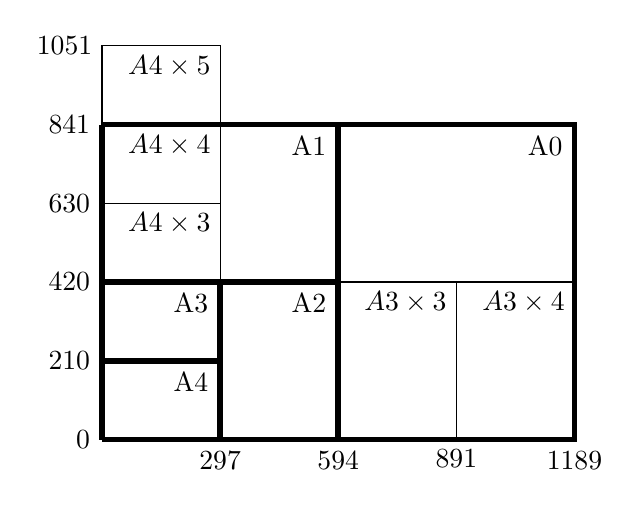
\begin{tikzpicture}
\draw[line width=0.7mm] (0,0)node[left]{0}--(0,1cm)node[left]{210}--(0,2cm)node[left]{420}--(0,3cm)node[left]{630}--(0,4cm)node[left]{841};
\draw(0,4cm)--(0,5cm)node[left]{1051}--(1.5cm,5cm)node[below left]{$A4\times 5$}--(1.5cm,2cm);
\draw[line width=0.7mm](0,1cm)--(1.5cm,1cm)node[below left]{A4}(0,2cm)--(1.5cm,2cm)node[below left]{A3}--(1.5cm,0)node[below]{297};
\draw(0,3cm)--(1.5cm,3cm)node[below left]{$A4\times 3$};
\draw[line width=0.7mm](0,4cm)--(3cm,4cm)node[below left]{A1}--(3cm,0)node[below]{594}(1.5cm,2cm)--(3cm,2cm)node[below left]{A2};
\draw[line width=0.7mm](3cm,4cm)--(6cm,4cm)node[below left]{A0}--(6cm,0)node[below]{1189}--(0,0);
\draw(3cm,2cm)--(4.5cm,2cm)node[below left]{$A3\times 3$}--(6cm,2cm)node[below left]{$A3\times 4$}(4.5cm,2cm)--(4.5cm,0)node[below]{891};
\draw(1.5cm,4cm)node[below left]{$A4\times 4$};
\end{tikzpicture}
\caption{图纸幅面及加长边} \label{fig:tufujiachang}
\end{figure}

从表\ref{tab:tufubiao1}中可以看出幅面之间的关系为:将A0图纸的长边对折后得到两张A1图纸,将A1图纸的长边对折后得到两纸A2图纸,以此类推。

\subsubsection{标题栏}
每张图样上必须画出标题栏,标题栏位于图样的右下角,与看图的方向一致。

标题栏分为更必区、签字区、名称及代号区和其他区,如图\ref{fig:biaotilan}所示。
\tikzset{
>=latex,
center lines/.style={dash pattern=on 20pt off 3pt on 2pt off 3pt},
importance lines/.style={line width=1pt}
}
\noindent
\begin{figure}[htbp]
\begin{tikzpicture}[scale=0.65]
\draw[line width=0.7mm](0,0)rectangle(180mm,56mm);
\draw(0,7mm)--(12mm,7mm)--(40mm,7mm)--++(40mm,0);
\draw(6mm,3.5mm)node{\tiny 工艺};
\draw(46mm,3.5mm)node{\tiny 批准};
\draw(0,14mm)--++(80mm,0);
\draw(6mm,10.5mm)node{\tiny 审核};
\draw(0,21mm)--++(12mm,0)--++(12mm,0)--++(16mm,0)--++(12mm,0)--++(12mm,0)--++(16mm,0);
\draw(6mm,24.5mm)node{\tiny设计};
\draw(18mm,24.5mm)node{\tiny(签名)};
\draw(32mm,24.5mm)node{\tiny(年月日)};
\draw(46mm,24.5mm)node{\tiny标准化};
\draw(58mm,24.5mm)node{\tiny签名};
\draw(72mm,24.5mm)node{\tiny(年月日)};
\draw(12mm,0)--++(0,28mm)(24mm,0)--++(0,28mm)(40mm,0)--++(0,28mm)(52mm,0)--++(0,28mm)(64mm,0)--++(0,28mm)(80mm,0)--++(0,28mm);
\draw(0,28mm)--++(10mm,0)--++(10mm,0)--++(16mm,0)--++(16mm,0)--++(12mm,0)--++(16mm,0);
\draw(5mm,31.5mm)node{\tiny 标记};
\draw(15mm,31.5mm)node{\tiny 处数};
\draw(28mm,31.5mm)node{\tiny 分区};
\draw(44mm,31.5mm)node{\tiny 更改文件号};
\draw(56mm,31.5mm)node{\tiny 签名};
\draw(72mm,31.5mm)node{\tiny 年月日};
\draw(0,35mm)--++(80mm,0)(0,42mm)--++(80mm,0)(0,49mm)--++(80mm,0);
\draw(10mm,28mm)--++(0,28mm)(20mm,28mm)--++(0,28mm)(36mm,28mm)--++(0,28mm)(52mm,28mm)--++(0,28mm)(64mm,28mm)--++(0,28mm)(80mm,28mm)--++(0,28mm);
\draw(80mm,9mm)--++(50mm,0);
\draw(105mm,4.5mm)node{\tiny 共\quad张\quad第\quad张};
\draw(80mm,18mm)--++(26mm,0)--++(12mm,0)--++(12mm,0);
\draw(93mm,23mm)node{\tiny 阶段标记};
\draw(112mm,23mm)node{\tiny 重量};
\draw(124mm,23mm)node{\tiny 比例};
\draw(86.5mm,9mm)--++(0,9mm)(93mm,9mm)--++(0,9mm)(99.5mm,9mm)--++(0,9mm)(106mm,9mm)--++(0,18mm)(118mm,9mm)--++(0,18mm);
\draw(80mm,28mm)--++(50mm,0);
\draw(130mm,0)--++(0,56mm);
\draw(130mm,18mm)--++(50mm,0)(130mm,38mm)--++(50mm,0);
\draw (155mm,9mm)node{\tiny(图样代号)};
\draw(155mm,28mm)node{\tiny(图样名称)};
\draw(155mm,48mm)node{\tiny(单位名称)};
\draw(105mm,48mm)node{\tiny(材料标记)};
\draw[<->](99.5mm,12mm)--(106mm,12mm)node[midway,above]{\tiny 6.5};
\draw(-14mm,0)--(0,0)(-7mm,7mm)--(0,7mm)(-14mm,56mm)--(0,56mm);
\draw[<->](-5mm,0)--(-5mm,7mm)node[midway,above,rotate=90]{\tiny 7};
\draw[<->](-13mm,0)--(-13mm,56mm)node[midway,above,rotate=90]{\tiny $8\times 7(56)$};
\draw(130mm,9mm)--++(9mm,0)(130mm,28mm)--++(9mm,0);
\draw[<->](137mm,0)--++(0,9mm)node[midway,above,rotate=90]{\tiny 9};
\draw[<->](137mm,9mm)--++(0,9mm)node[midway,above,rotate=90]{\tiny 9};
\draw[<->](137mm,18mm)--++(0,10mm)node[midway,above,rotate=90]{\tiny 10};
\draw(180mm,0)--++(9mm,0)(180mm,18mm)--++(9mm,0)(180mm,38mm)--++(9mm,0);
\draw[<->](187mm,0)--++(0,18mm)node[midway,above,rotate=90]{\tiny 18};
\draw[<->](187mm,18mm)--++(0,20mm)node[midway,above,rotate=90]{\tiny 20};
\draw(0,-9mm)--++(0,9mm)(12mm,-9mm)--++(0,9mm)(24mm,-9mm)--++(0,9mm)(40mm,-9mm)--++(0,9mm)(52mm,-9mm)--++(0,9mm)(64mm,-9mm)--++(0,9mm)(80mm,-9mm)--++(0,9mm)(130mm,-9mm)--++(0,9mm);
\draw[<->](0,-7mm)--++(12mm,0)node[midway,above]{\tiny 12};
\draw[<->](12mm,-7mm)--++(12mm,0)node[midway,above]{\tiny 12};
\draw[<->](24mm,-7mm)--++(16mm,0)node[midway,above]{\tiny 16};
\draw[<->](40mm,-7mm)--++(12mm,0)node[midway,above]{\tiny 12};
\draw[<->](52mm,-7mm)--++(12mm,0)node[midway,above]{\tiny 12};
\draw[<->](64mm,-7mm)--++(16mm,0)node[midway,above]{\tiny 16};
\draw[<->](80mm,-7mm)--++(50mm,0)node[midway,above]{\tiny 50};
\draw(0,-18mm)--(0,0)(180mm,-18mm)--(180mm,0);
\draw[<->](0,-16mm)--(180mm,-16mm)node[midway,above]{\tiny 180};
\draw(0,56mm)--++(0,7mm)(10mm,56mm)--++(0,7mm)(20mm,56mm)--++(0,7mm)(36mm,56mm)--++(0,7mm)(52mm,56mm)--++(0,7mm)(64mm,56mm)--++(0,7mm)(80mm,56mm)--++(0,7mm);
\draw[<->](0,61mm)--++(10mm,0)node[midway,above]{\tiny 10};
\draw[<->](10mm,61mm)--++(10mm,0)node[midway,above]{\tiny 10};
\draw[<->](20mm,61mm)--++(16mm,0)node[midway,above]{\tiny 16};
\draw[<->](36mm,61mm)--++(16mm,0)node[midway,above]{\tiny 16};
\draw[<->](52mm,61mm)--++(12mm,0)node[midway,above]{\tiny 12};
\draw[<->](64mm,61mm)--++(16mm,0)node[midway,above]{\tiny 16};
\draw(106mm,28mm)--++(0,7mm)(118mm,28mm)--++(0,7mm);
\draw[<->](80mm,33mm)--++(26mm,0)node[midway,above]{\tiny $4\times 6.5(26)$};
\draw[<->](106mm,33mm)--++(12mm,0)node[midway,above]{\tiny 12};
\draw[<->](118mm,33mm)--++(12mm,0)node[midway,above]{\tiny 12};
\end{tikzpicture}
\caption{标题栏格式及尺寸}\label{fig:biaotilan}
\end{figure}

\begin{figure}[htbp]
\centering
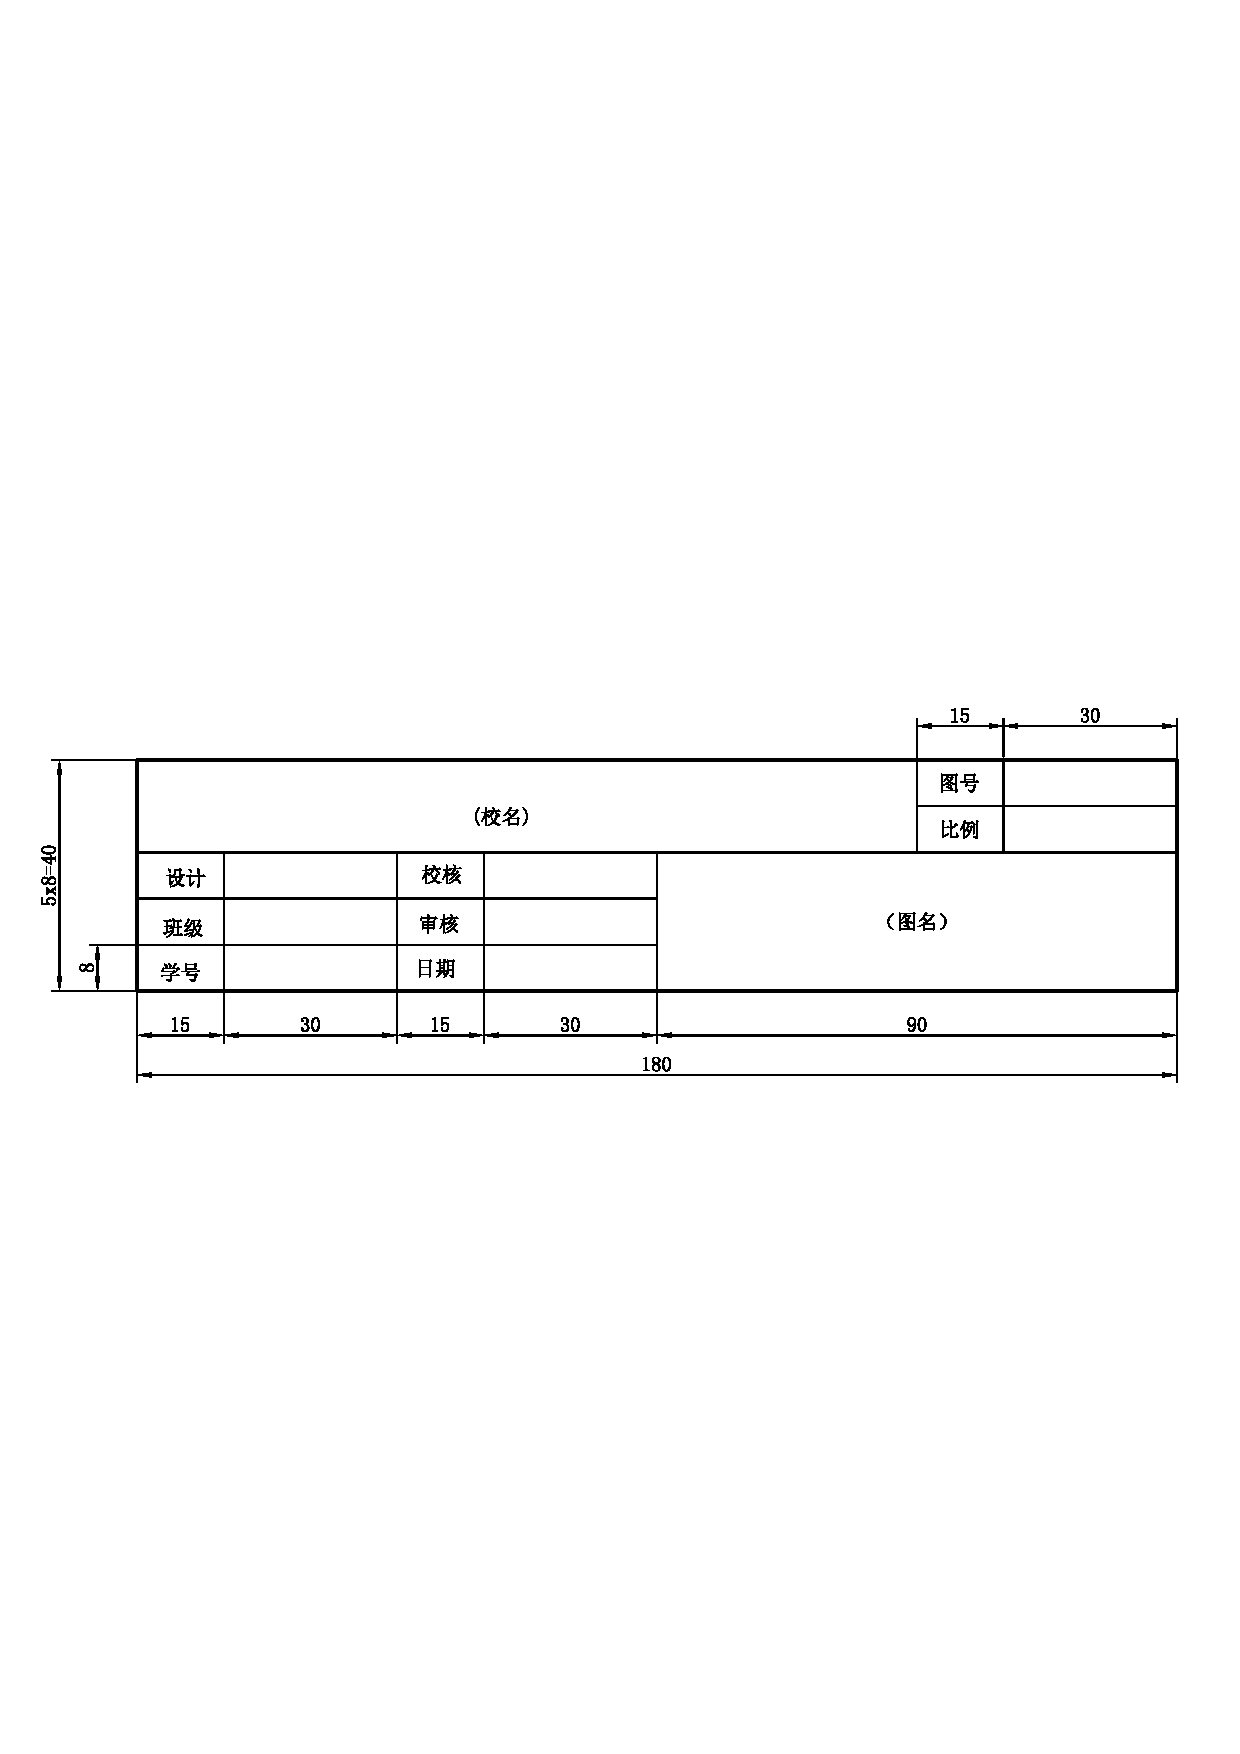
\includegraphics[scale=0.65]{biaotilan.pdf}
\caption{学生用标题栏格式及尺寸}\label{fig:biaotilan1}
\end{figure}
\indent

\subsubsection{图框格式}
图框格式分为留装订边和不留装订边两种,其装订边尺寸如表\ref{tab:tufubiao1}所示。图\ref{fig:zhuangding}所示为采用A4幅面竖装和A3幅面横装时,留装订边和不留装订边的图框格式。
\noindent
\tikzset{
>=latex,
center lines/.style={dash pattern=on 20pt off 3pt on 2pt off 3pt},
importance lines/.style={line width=1pt}
}
\begin{figure}[htbp]
\centering
\subfloat[留装订边格式]{
\begin{tikzpicture}
\draw(0,0)rectangle(4cm,5cm);
\draw[line width=0.7mm](0.5cm,0.25cm)rectangle(3.75cm,4.75cm)(1.5cm,0.25cm)--(1.5cm,1cm)--(3.75cm,1cm)node[midway,below]{标题栏};
\draw(-0.7cm,0)--(0,0)(-0.7cm,5cm)--(0cm,5cm);
\draw[<->](-0.5cm,0)--(-0.5cm,5cm)node[midway,above,rotate=90]{$L$};
\draw(0,-0.7cm)--(0,0)(4cm,-0.7cm)--(4cm,0);
\draw[<->](0,-0.5cm)--(4cm,-0.5cm)node[midway,above]{$B$};
\draw[->](1cm,-0.45cm)--(1cm,0);
\draw[->](1cm,0.65cm)--(1cm,0.25cm)node[midway,above,rotate=90]{$c$};
\draw(1cm,0)--(1cm,0.25cm);
\draw[->](-0.4cm,2cm)--(0,2cm);
\draw[->](0.9cm,2cm)--(0.5cm,2cm);
\draw(0,2cm)--(0.5cm,2cm)node[midway,above]{$a$};
\draw[->](2cm,5cm)--(2cm,4.35cm)--(2cm,4.75cm);
\draw[->](2cm,5.45cm)--(2cm,5cm)node[midway,above,rotate=90]{$c$};
\draw[->](4cm,2.5cm)--(3.3cm,2.5cm)--(3.75cm,2.5cm);
\draw[->](4.45cm,2.5cm)--(4cm,2.5cm)node[midway,above]{$c$};

\begin{scope}[xshift=5.5cm]
\draw(0,0)rectangle(7cm,5cm);
\draw[line width=0.7mm](0.5cm,0.25cm)rectangle(6.75cm,4.75cm)(4.5cm,0.25cm)--(4.5cm,1cm)--(6.75cm,1cm)node[midway,below]{标题栏};
\draw(-0.7cm,0)--(0,0)(-0.7cm,5cm)--(0cm,5cm);
\draw[<->](-0.5cm,0)--(-0.5cm,5cm)node[midway,above,rotate=90]{$B$};
\draw(0,-0.7cm)--(0,0)(7cm,-0.7cm)--(7cm,0);
\draw[<->](0,-0.5cm)--(7cm,-0.5cm)node[midway,above]{$L$};
\draw[->](3cm,-0.45cm)--(3cm,0);
\draw[->](3cm,0.65cm)--(3cm,0.25cm)node[midway,above,rotate=90]{$c$};
\draw(3cm,0)--(3cm,0.25cm);
\draw[->](-0.4cm,2cm)--(0,2cm);
\draw[->](0.9cm,2cm)--(0.5cm,2cm);
\draw(0,2cm)--(0.5cm,2cm)node[midway,above]{$a$};
\draw[->](3.5cm,5cm)--(3.5cm,4.35cm)--(3.5cm,4.75cm);
\draw[->](3.5cm,5.45cm)--(3.5cm,5cm)node[midway,above,rotate=90]{$c$};
\draw[->](7cm,2.5cm)--(6.3cm,2.5cm)--(6.75cm,2.5cm);
\draw[->](7.45cm,2.5cm)--(7cm,2.5cm)node[midway,above]{$c$};
\end{scope}
\end{tikzpicture}}

\subfloat[不留装订边格式]{
\begin{tikzpicture}
\draw(0,0)rectangle(4cm,5cm);
\draw[line width=0.7mm](0.25cm,0.25cm)rectangle(3.75cm,4.75cm)(1.5cm,0.25cm)--(1.5cm,1cm)--(3.75cm,1cm)node[midway,below]{标题栏};
\draw(-0.7cm,0)--(0,0)(-0.7cm,5cm)--(0cm,5cm);
\draw[<->](-0.5cm,0)--(-0.5cm,5cm)node[midway,above,rotate=90]{$L$};
\draw(0,-0.7cm)--(0,0)(4cm,-0.7cm)--(4cm,0);
\draw[<->](0,-0.5cm)--(4cm,-0.5cm)node[midway,above]{$B$};
\draw[->](1cm,-0.45cm)--(1cm,0);
\draw[->](1cm,0.65cm)--(1cm,0.25cm)node[midway,above,rotate=90]{$c$};
\draw(1cm,0)--(1cm,0.25cm);
\draw[->](-0.4cm,2cm)--(0,2cm);
\draw[->](0.65cm,2cm)--(0.25cm,2cm)node[midway,above]{$c$};
\draw(0,2cm)--(0.25cm,2cm);
\draw[->](2cm,5cm)--(2cm,4.35cm)--(2cm,4.75cm);
\draw[->](2cm,5.45cm)--(2cm,5cm)node[midway,above,rotate=90]{$c$};
\draw[->](4cm,2.5cm)--(3.3cm,2.5cm)--(3.75cm,2.5cm);
\draw[->](4.45cm,2.5cm)--(4cm,2.5cm)node[midway,above]{$c$};

\begin{scope}[xshift=5.5cm]
\draw(0,0)rectangle(7cm,5cm);
\draw[line width=0.7mm](0.25cm,0.25cm)rectangle(6.75cm,4.75cm)(4.5cm,0.25cm)--(4.5cm,1cm)--(6.75cm,1cm)node[midway,below]{标题栏};
\draw(-0.7cm,0)--(0,0)(-0.7cm,5cm)--(0cm,5cm);
\draw[<->](-0.5cm,0)--(-0.5cm,5cm)node[midway,above,rotate=90]{$B$};
\draw(0,-0.7cm)--(0,0)(7cm,-0.7cm)--(7cm,0);
\draw[<->](0,-0.5cm)--(7cm,-0.5cm)node[midway,above]{$L$};
\draw[->](3cm,-0.45cm)--(3cm,0);
\draw[->](3cm,0.65cm)--(3cm,0.25cm)node[midway,above,rotate=90]{$c$};
\draw(3cm,0)--(3cm,0.25cm);
\draw[->](-0.4cm,2cm)--(0,2cm);
\draw[->](0.65cm,2cm)--(0.25cm,2cm)node[midway,above]{$c$};
\draw(0,2cm)--(0.25cm,2cm);
\draw[->](3.5cm,5cm)--(3.5cm,4.35cm)--(3.5cm,4.75cm);
\draw[->](3.5cm,5.45cm)--(3.5cm,5cm)node[midway,above,rotate=90]{$c$};
\draw[->](7cm,2.5cm)--(6.3cm,2.5cm)--(6.75cm,2.5cm);
\draw[->](7.45cm,2.5cm)--(7cm,2.5cm)node[midway,above]{$c$};
\end{scope}
\end{tikzpicture}}
\caption{图框格式}\label{fig:zhuangding}
\end{figure}
\indent

\section{小结}

\endinput